\documentclass[twoside]{book}

% Packages required by doxygen
\usepackage{fixltx2e}
\usepackage{calc}
\usepackage{doxygen}
\usepackage{graphicx}
\usepackage[utf8]{inputenc}
\usepackage{makeidx}
\usepackage{multicol}
\usepackage{multirow}
\PassOptionsToPackage{warn}{textcomp}
\usepackage{textcomp}
\usepackage[nointegrals]{wasysym}
\usepackage[table]{xcolor}

% Font selection
\usepackage[T1]{fontenc}
\usepackage{mathptmx}
\usepackage[scaled=.90]{helvet}
\usepackage{courier}
\usepackage{amssymb}
\usepackage{sectsty}
\renewcommand{\familydefault}{\sfdefault}
\allsectionsfont{%
  \fontseries{bc}\selectfont%
  \color{darkgray}%
}
\renewcommand{\DoxyLabelFont}{%
  \fontseries{bc}\selectfont%
  \color{darkgray}%
}
\newcommand{\+}{\discretionary{\mbox{\scriptsize$\hookleftarrow$}}{}{}}

% Page & text layout
\usepackage{geometry}
\geometry{%
  a4paper,%
  top=2.5cm,%
  bottom=2.5cm,%
  left=2.5cm,%
  right=2.5cm%
}
\tolerance=750
\hfuzz=15pt
\hbadness=750
\setlength{\emergencystretch}{15pt}
\setlength{\parindent}{0cm}
\setlength{\parskip}{0.2cm}
\makeatletter
\renewcommand{\paragraph}{%
  \@startsection{paragraph}{4}{0ex}{-1.0ex}{1.0ex}{%
    \normalfont\normalsize\bfseries\SS@parafont%
  }%
}
\renewcommand{\subparagraph}{%
  \@startsection{subparagraph}{5}{0ex}{-1.0ex}{1.0ex}{%
    \normalfont\normalsize\bfseries\SS@subparafont%
  }%
}
\makeatother

% Headers & footers
\usepackage{fancyhdr}
\pagestyle{fancyplain}
\fancyhead[LE]{\fancyplain{}{\bfseries\thepage}}
\fancyhead[CE]{\fancyplain{}{}}
\fancyhead[RE]{\fancyplain{}{\bfseries\leftmark}}
\fancyhead[LO]{\fancyplain{}{\bfseries\rightmark}}
\fancyhead[CO]{\fancyplain{}{}}
\fancyhead[RO]{\fancyplain{}{\bfseries\thepage}}
\fancyfoot[LE]{\fancyplain{}{}}
\fancyfoot[CE]{\fancyplain{}{}}
\fancyfoot[RE]{\fancyplain{}{\bfseries\scriptsize Generated on Fri Oct 17 2014 13\+:28\+:08 for Typing Tutor by Doxygen }}
\fancyfoot[LO]{\fancyplain{}{\bfseries\scriptsize Generated on Fri Oct 17 2014 13\+:28\+:08 for Typing Tutor by Doxygen }}
\fancyfoot[CO]{\fancyplain{}{}}
\fancyfoot[RO]{\fancyplain{}{}}
\renewcommand{\footrulewidth}{0.4pt}
\renewcommand{\chaptermark}[1]{%
  \markboth{#1}{}%
}
\renewcommand{\sectionmark}[1]{%
  \markright{\thesection\ #1}%
}

% Indices & bibliography
\usepackage{natbib}
\usepackage[titles]{tocloft}
\setcounter{tocdepth}{3}
\setcounter{secnumdepth}{5}
\makeindex

% Hyperlinks (required, but should be loaded last)
\usepackage{ifpdf}
\ifpdf
  \usepackage[pdftex,pagebackref=true]{hyperref}
\else
  \usepackage[ps2pdf,pagebackref=true]{hyperref}
\fi
\hypersetup{%
  colorlinks=true,%
  linkcolor=blue,%
  citecolor=blue,%
  unicode%
}

% Custom commands
\newcommand{\clearemptydoublepage}{%
  \newpage{\pagestyle{empty}\cleardoublepage}%
}


%===== C O N T E N T S =====

\begin{document}

% Titlepage & ToC
\hypersetup{pageanchor=false,
             bookmarks=true,
             bookmarksnumbered=true,
             pdfencoding=unicode
            }
\pagenumbering{roman}
\begin{titlepage}
\vspace*{7cm}
\begin{center}%
{\Large Typing Tutor }\\
\vspace*{1cm}
{\large Generated by Doxygen 1.8.8}\\
\vspace*{0.5cm}
{\small Fri Oct 17 2014 13:28:08}\\
\end{center}
\end{titlepage}
\clearemptydoublepage
\tableofcontents
\clearemptydoublepage
\pagenumbering{arabic}
\hypersetup{pageanchor=true}

%--- Begin generated contents ---
\chapter{typingtutor}
\label{md__r_e_a_d_m_e}
\hypertarget{md__r_e_a_d_m_e}{}
A simple typing tutor which uses text files as exercises. 
\chapter{Hierarchical Index}
\section{Class Hierarchy}
This inheritance list is sorted roughly, but not completely, alphabetically\+:\begin{DoxyCompactList}
\item Frame\begin{DoxyCompactList}
\item \contentsline{section}{main.\+Main\+Frame}{\pageref{classmain_1_1_main_frame}}{}
\end{DoxyCompactList}
\item Text\+Ctrl\begin{DoxyCompactList}
\item \contentsline{section}{main.\+My\+Text\+Ctrl}{\pageref{classmain_1_1_my_text_ctrl}}{}
\end{DoxyCompactList}
\end{DoxyCompactList}

\chapter{Class Index}
\section{Class List}
Here are the classes, structs, unions and interfaces with brief descriptions\+:\begin{DoxyCompactList}
\item\contentsline{section}{\hyperlink{classmain_1_1_main_frame}{main.\+Main\+Frame} }{\pageref{classmain_1_1_main_frame}}{}
\item\contentsline{section}{\hyperlink{classmain_1_1_my_text_ctrl}{main.\+My\+Text\+Ctrl} }{\pageref{classmain_1_1_my_text_ctrl}}{}
\end{DoxyCompactList}

\chapter{Class Documentation}
\hypertarget{classmain_1_1_main_frame}{\section{main.\+Main\+Frame Class Reference}
\label{classmain_1_1_main_frame}\index{main.\+Main\+Frame@{main.\+Main\+Frame}}
}
Inheritance diagram for main.\+Main\+Frame\+:\begin{figure}[H]
\begin{center}
\leavevmode
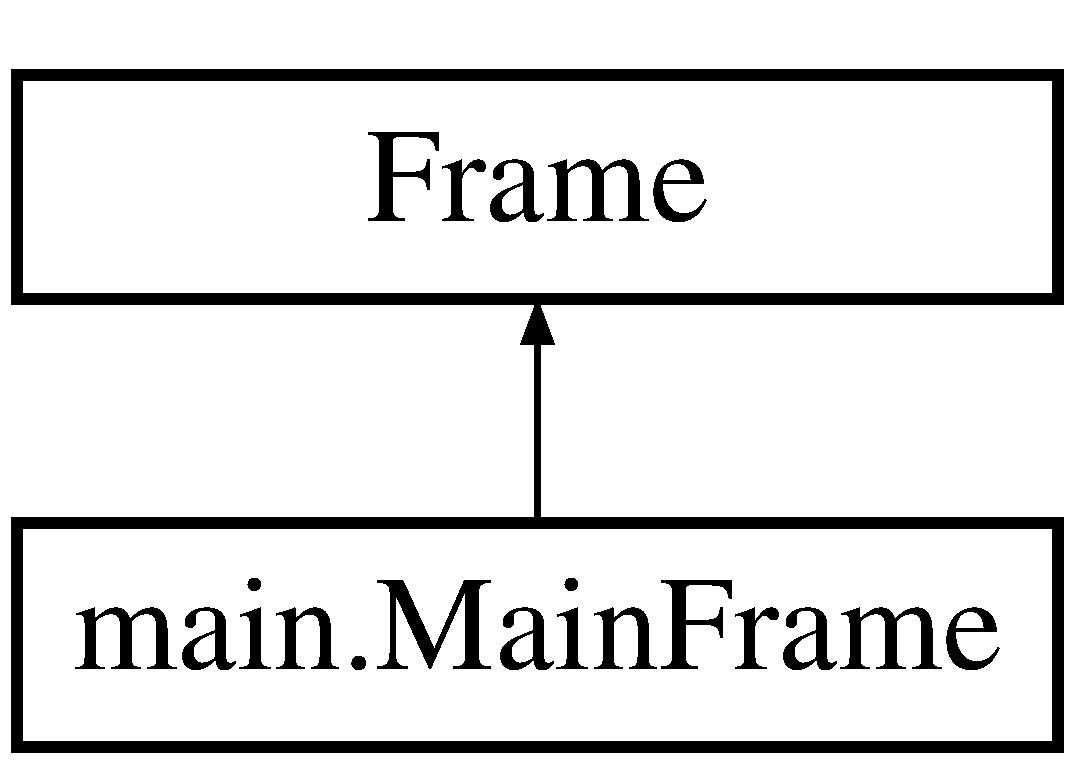
\includegraphics[height=2.000000cm]{classmain_1_1_main_frame}
\end{center}
\end{figure}
\subsection*{Public Member Functions}
\begin{DoxyCompactItemize}
\item 
def \hyperlink{classmain_1_1_main_frame_a03cf7833edb9fa538844710f9ff5a8aa}{\+\_\+\+\_\+init\+\_\+\+\_\+}
\item 
\hypertarget{classmain_1_1_main_frame_aa9bd704144c614aaf4586d2cd2b3d8be}{def {\bfseries get\+Verbose}}\label{classmain_1_1_main_frame_aa9bd704144c614aaf4586d2cd2b3d8be}

\item 
\hypertarget{classmain_1_1_main_frame_a0f583715f1e4d919e1868d9df38c3d83}{def {\bfseries set\+Verbose}}\label{classmain_1_1_main_frame_a0f583715f1e4d919e1868d9df38c3d83}

\item 
\hypertarget{classmain_1_1_main_frame_a2df2d8c821da4aa4c52c7534e824d69b}{def {\bfseries get\+Keyboard\+Helper}}\label{classmain_1_1_main_frame_a2df2d8c821da4aa4c52c7534e824d69b}

\item 
\hypertarget{classmain_1_1_main_frame_ad6840582e953002cb0ab94fec037fc32}{def {\bfseries set\+Keyboard\+Helper}}\label{classmain_1_1_main_frame_ad6840582e953002cb0ab94fec037fc32}

\item 
\hypertarget{classmain_1_1_main_frame_a2b7bb3f0041af126d27f58c41e7239ac}{def {\bfseries get\+Play\+Sounds}}\label{classmain_1_1_main_frame_a2b7bb3f0041af126d27f58c41e7239ac}

\item 
\hypertarget{classmain_1_1_main_frame_abf041b8e926dd9fa0a522463d5000de3}{def {\bfseries set\+Play\+Sounds}}\label{classmain_1_1_main_frame_abf041b8e926dd9fa0a522463d5000de3}

\item 
\hypertarget{classmain_1_1_main_frame_acafee3190e194ab1b585e77dcacc2072}{def {\bfseries sound}}\label{classmain_1_1_main_frame_acafee3190e194ab1b585e77dcacc2072}

\item 
\hypertarget{classmain_1_1_main_frame_a6b700a95a83900eea614f2b3837e1259}{def {\bfseries get\+Current\+Letter}}\label{classmain_1_1_main_frame_a6b700a95a83900eea614f2b3837e1259}

\item 
\hypertarget{classmain_1_1_main_frame_a9eaf9c8f88f50ecddcf57d873de6f903}{def {\bfseries process\+Key}}\label{classmain_1_1_main_frame_a9eaf9c8f88f50ecddcf57d873de6f903}

\item 
\hypertarget{classmain_1_1_main_frame_a820dd5e824f215864b9bd0d9083664b2}{def {\bfseries open\+File}}\label{classmain_1_1_main_frame_a820dd5e824f215864b9bd0d9083664b2}

\item 
\hypertarget{classmain_1_1_main_frame_a64fd468283e1c15833cb5e32d5379371}{def {\bfseries start\+Tutor}}\label{classmain_1_1_main_frame_a64fd468283e1c15833cb5e32d5379371}

\item 
\hypertarget{classmain_1_1_main_frame_a3ed49300a9b18da06050898eed44e7cd}{def {\bfseries toggle\+Verbosity}}\label{classmain_1_1_main_frame_a3ed49300a9b18da06050898eed44e7cd}

\item 
\hypertarget{classmain_1_1_main_frame_a1cf2fa165b18baf7bef50a786df04d12}{def {\bfseries toggle\+Mute}}\label{classmain_1_1_main_frame_a1cf2fa165b18baf7bef50a786df04d12}

\item 
\hypertarget{classmain_1_1_main_frame_a5cdc95fcd25ebc2e57e8b1b510db8a09}{def {\bfseries On\+Close}}\label{classmain_1_1_main_frame_a5cdc95fcd25ebc2e57e8b1b510db8a09}

\item 
\hypertarget{classmain_1_1_main_frame_ae06508af0aa46c0e304507b40a9ae403}{def {\bfseries volume\+Down}}\label{classmain_1_1_main_frame_ae06508af0aa46c0e304507b40a9ae403}

\item 
\hypertarget{classmain_1_1_main_frame_a977058d31d385a7dc55d7585145732b4}{def {\bfseries volume\+Up}}\label{classmain_1_1_main_frame_a977058d31d385a7dc55d7585145732b4}

\item 
\hypertarget{classmain_1_1_main_frame_af807db0d3f970b27cc6b5a0ba5a976ef}{def {\bfseries set\+Volume}}\label{classmain_1_1_main_frame_af807db0d3f970b27cc6b5a0ba5a976ef}

\item 
def \hyperlink{classmain_1_1_main_frame_ae6f49c760b795f578b9994b1922ecd05}{quit}
\item 
def \hyperlink{classmain_1_1_main_frame_a62b3e7925250b4603c967d6895a2519b}{about}
\end{DoxyCompactItemize}
\subsection*{Public Attributes}
\begin{DoxyCompactItemize}
\item 
\hypertarget{classmain_1_1_main_frame_a74d69b9333c27fe6d4f9139f7c5c1f82}{{\bfseries tutor\+Index}}\label{classmain_1_1_main_frame_a74d69b9333c27fe6d4f9139f7c5c1f82}

\item 
\hypertarget{classmain_1_1_main_frame_a28011140dba0f8e2e947a3591840504c}{{\bfseries file\+Contents}}\label{classmain_1_1_main_frame_a28011140dba0f8e2e947a3591840504c}

\item 
\hypertarget{classmain_1_1_main_frame_adaaeafe2b7295d1312d00c0c0d05ea5a}{{\bfseries mistakes}}\label{classmain_1_1_main_frame_adaaeafe2b7295d1312d00c0c0d05ea5a}

\item 
\hypertarget{classmain_1_1_main_frame_a22e8029065c06ac730cbe5d964458e74}{{\bfseries started}}\label{classmain_1_1_main_frame_a22e8029065c06ac730cbe5d964458e74}

\item 
\hypertarget{classmain_1_1_main_frame_a6ef5d668539081684c72da05deacbbc6}{{\bfseries finished}}\label{classmain_1_1_main_frame_a6ef5d668539081684c72da05deacbbc6}

\item 
\hypertarget{classmain_1_1_main_frame_ac81eb129666f11a4ce1574884b5f6c42}{{\bfseries label}}\label{classmain_1_1_main_frame_ac81eb129666f11a4ce1574884b5f6c42}

\item 
\hypertarget{classmain_1_1_main_frame_a718d5aa6cc6cca8dd84a18c6df1a7eef}{{\bfseries entry}}\label{classmain_1_1_main_frame_a718d5aa6cc6cca8dd84a18c6df1a7eef}

\end{DoxyCompactItemize}


\subsection{Detailed Description}
\begin{DoxyVerb}This is the main window of the program.\end{DoxyVerb}
 

\subsection{Constructor \& Destructor Documentation}
\hypertarget{classmain_1_1_main_frame_a03cf7833edb9fa538844710f9ff5a8aa}{\index{main\+::\+Main\+Frame@{main\+::\+Main\+Frame}!\+\_\+\+\_\+init\+\_\+\+\_\+@{\+\_\+\+\_\+init\+\_\+\+\_\+}}
\index{\+\_\+\+\_\+init\+\_\+\+\_\+@{\+\_\+\+\_\+init\+\_\+\+\_\+}!main\+::\+Main\+Frame@{main\+::\+Main\+Frame}}
\subsubsection[{\+\_\+\+\_\+init\+\_\+\+\_\+}]{\setlength{\rightskip}{0pt plus 5cm}def main.\+Main\+Frame.\+\_\+\+\_\+init\+\_\+\+\_\+ (
\begin{DoxyParamCaption}
\item[{}]{self}
\end{DoxyParamCaption}
)}}\label{classmain_1_1_main_frame_a03cf7833edb9fa538844710f9ff5a8aa}
\begin{DoxyVerb}Construct the class.\end{DoxyVerb}
 

\subsection{Member Function Documentation}
\hypertarget{classmain_1_1_main_frame_a62b3e7925250b4603c967d6895a2519b}{\index{main\+::\+Main\+Frame@{main\+::\+Main\+Frame}!about@{about}}
\index{about@{about}!main\+::\+Main\+Frame@{main\+::\+Main\+Frame}}
\subsubsection[{about}]{\setlength{\rightskip}{0pt plus 5cm}def main.\+Main\+Frame.\+about (
\begin{DoxyParamCaption}
\item[{}]{self, }
\item[{}]{event}
\end{DoxyParamCaption}
)}}\label{classmain_1_1_main_frame_a62b3e7925250b4603c967d6895a2519b}
\begin{DoxyVerb}Show an about dialog, and give the user the option to visit the website.\end{DoxyVerb}
 \hypertarget{classmain_1_1_main_frame_ae6f49c760b795f578b9994b1922ecd05}{\index{main\+::\+Main\+Frame@{main\+::\+Main\+Frame}!quit@{quit}}
\index{quit@{quit}!main\+::\+Main\+Frame@{main\+::\+Main\+Frame}}
\subsubsection[{quit}]{\setlength{\rightskip}{0pt plus 5cm}def main.\+Main\+Frame.\+quit (
\begin{DoxyParamCaption}
\item[{}]{self, }
\item[{}]{event}
\end{DoxyParamCaption}
)}}\label{classmain_1_1_main_frame_ae6f49c760b795f578b9994b1922ecd05}
\begin{DoxyVerb}Quits the program.\end{DoxyVerb}
 

The documentation for this class was generated from the following file\+:\begin{DoxyCompactItemize}
\item 
main.\+py\end{DoxyCompactItemize}

\hypertarget{classmain_1_1_my_text_ctrl}{\section{main.\+My\+Text\+Ctrl Class Reference}
\label{classmain_1_1_my_text_ctrl}\index{main.\+My\+Text\+Ctrl@{main.\+My\+Text\+Ctrl}}
}
Inheritance diagram for main.\+My\+Text\+Ctrl\+:\begin{figure}[H]
\begin{center}
\leavevmode
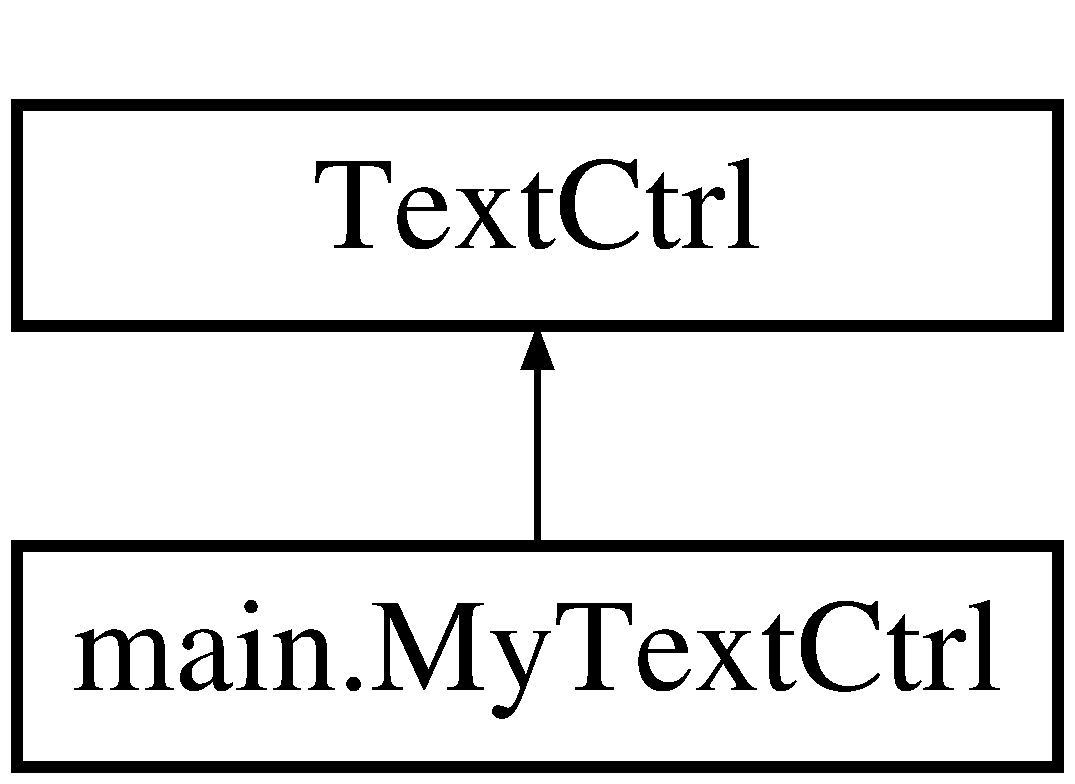
\includegraphics[height=2.000000cm]{classmain_1_1_my_text_ctrl}
\end{center}
\end{figure}
\subsection*{Public Member Functions}
\begin{DoxyCompactItemize}
\item 
def \hyperlink{classmain_1_1_my_text_ctrl_a3cb37d241a38f106aac793df70d151a1}{\+\_\+\+\_\+init\+\_\+\+\_\+}
\item 
def \hyperlink{classmain_1_1_my_text_ctrl_a8f6317decefa9ddff5dceea1288156a0}{Set\+Value}
\end{DoxyCompactItemize}


\subsection{Detailed Description}
\begin{DoxyVerb}This class is used so that every time tehe value gets set, the cursor is jumped to the end, instead of the beginning (which is the wx default).\end{DoxyVerb}
 

\subsection{Constructor \& Destructor Documentation}
\hypertarget{classmain_1_1_my_text_ctrl_a3cb37d241a38f106aac793df70d151a1}{\index{main\+::\+My\+Text\+Ctrl@{main\+::\+My\+Text\+Ctrl}!\+\_\+\+\_\+init\+\_\+\+\_\+@{\+\_\+\+\_\+init\+\_\+\+\_\+}}
\index{\+\_\+\+\_\+init\+\_\+\+\_\+@{\+\_\+\+\_\+init\+\_\+\+\_\+}!main\+::\+My\+Text\+Ctrl@{main\+::\+My\+Text\+Ctrl}}
\subsubsection[{\+\_\+\+\_\+init\+\_\+\+\_\+}]{\setlength{\rightskip}{0pt plus 5cm}def main.\+My\+Text\+Ctrl.\+\_\+\+\_\+init\+\_\+\+\_\+ (
\begin{DoxyParamCaption}
\item[{}]{self, }
\item[{}]{panel}
\end{DoxyParamCaption}
)}}\label{classmain_1_1_my_text_ctrl_a3cb37d241a38f106aac793df70d151a1}
\begin{DoxyVerb}Set up the class with the provided panel. Fill in all other values automatically.\end{DoxyVerb}
 

\subsection{Member Function Documentation}
\hypertarget{classmain_1_1_my_text_ctrl_a8f6317decefa9ddff5dceea1288156a0}{\index{main\+::\+My\+Text\+Ctrl@{main\+::\+My\+Text\+Ctrl}!Set\+Value@{Set\+Value}}
\index{Set\+Value@{Set\+Value}!main\+::\+My\+Text\+Ctrl@{main\+::\+My\+Text\+Ctrl}}
\subsubsection[{Set\+Value}]{\setlength{\rightskip}{0pt plus 5cm}def main.\+My\+Text\+Ctrl.\+Set\+Value (
\begin{DoxyParamCaption}
\item[{}]{self, }
\item[{}]{value}
\end{DoxyParamCaption}
)}}\label{classmain_1_1_my_text_ctrl_a8f6317decefa9ddff5dceea1288156a0}
\begin{DoxyVerb}Set the value as per usual, then move the insertion point to the end.\end{DoxyVerb}
 

The documentation for this class was generated from the following file\+:\begin{DoxyCompactItemize}
\item 
main.\+py\end{DoxyCompactItemize}

%--- End generated contents ---

% Index
\newpage
\phantomsection
\addcontentsline{toc}{chapter}{Index}
\printindex

\end{document}
